% MATS poster session — 36x24in landscape, beamerposter.
% Build: lualatex poster.tex  (from this directory)
% Proof: pdftoppm -png -r 30 poster.pdf proof && open proof-1.png
\documentclass[final]{beamer}
\usepackage[orientation=landscape,size=custom,width=91.44,height=60.96,scale=0.95]{beamerposter}
\usepackage{lmodern}
\usepackage[T1]{fontenc}
\usepackage{graphicx}
\usepackage{amsmath}
\graphicspath{{figures/}}

% ---------- colors (MATS-ish: deep navy banner, teal accents) ----------
\definecolor{banner}{RGB}{16,42,67}
\definecolor{accent}{RGB}{0,114,178}
\definecolor{blockbg}{RGB}{245,247,250}
\definecolor{takeaway}{RGB}{0,94,70}

\setbeamercolor{headline}{bg=banner,fg=white}
\setbeamercolor{block title}{fg=white,bg=accent}
\setbeamercolor{block body}{fg=black,bg=blockbg}
\setbeamertemplate{navigation symbols}{}
\setbeamerfont{block title}{size=\large,series=\bfseries}
\setbeamertemplate{itemize item}{\color{accent}$\blacktriangleright$}
\setlength{\parskip}{0.25em}

\newcommand{\vC}{\ensuremath{v_C}}
\newcommand{\vA}{\ensuremath{v_A}}
\newcommand{\takeaways}[1]{{\color{takeaway}\textbf{#1}}}

% Block with reduced vertical padding
\setbeamertemplate{block begin}{
  \vskip.3ex
  \begin{beamercolorbox}[rounded=true,leftskip=0.5em,colsep*=.5ex]{block title}
    \usebeamerfont{block title}\insertblocktitle
  \end{beamercolorbox}
  {\parskip0pt\par}
  \usebeamerfont{block body}
  \begin{beamercolorbox}[rounded=true,colsep*=.5ex,sep=.4ex,vmode]{block body}
}
\setbeamertemplate{block end}{\end{beamercolorbox}\vskip.3ex}

\begin{document}
\begin{frame}[t]

% ==================== TITLE BANNER ====================
\begin{beamercolorbox}[wd=\paperwidth,sep=0.55em]{headline}
  \centering
  {\Huge\bfseries The Surprising Effectiveness of Linear Context-to-Answer Maps in Language Models\\[0.3em]}
  {\normalsize
    Thomas Jiralerspong$^{1,2}$ \quad
    Christopher Ackerman$^{2}$ \quad
    Mukesh Ramanathan$^{2}$ \quad
    Christina Lu$^{3}$ \quad
    Guillaume Lajoie$^{1}$ \quad
    Dan Mossing$^{3}$
    \qquad\quad
    {\color{white!80!banner}$^{1}$Mila, Universit\'e de Montr\'eal \quad $^{2}$MATS \quad $^{3}$Anthropic}
  }
\end{beamercolorbox}

\vskip0.4em

\begin{columns}[t]

% ==================== COLUMN 1 ====================
\begin{column}{0.24\textwidth}

\begin{block}{Motivation}
Absent external inputs, an LLM's entire answer distribution is \textbf{fixed before the first answer token is generated}: the model is a deterministic mapping from context to answer distribution. A cheap approximation of it would predict behavior pre-generation and anticipate fine-tuning effects. Prior work gives \emph{cheap but narrow} predictors (single tokens, activations, behaviors) or a \emph{whole-distribution but expensive} imitator (distillation). Can we cheaply approximate the mapping \emph{as a whole}?
\end{block}

\begin{block}{The residual context-answer mapping}
\begin{center}

\includegraphics[width=0.99\linewidth]{fig1_schematic.pdf}
\end{center}
A minimal \textbf{metamodel} in activation space: the \textbf{context vector} \vC{} (residual-stream state at the last context token, layer $\ell$) is mapped to the \textbf{answer vector} \vA{} (mean answer-token activation). We fit $\vC \mapsto \vA$ maps across models, families, post-training stages, and corpora.
\end{block}

\begin{block}{1. High predictive power, mostly linear}
\begin{center}
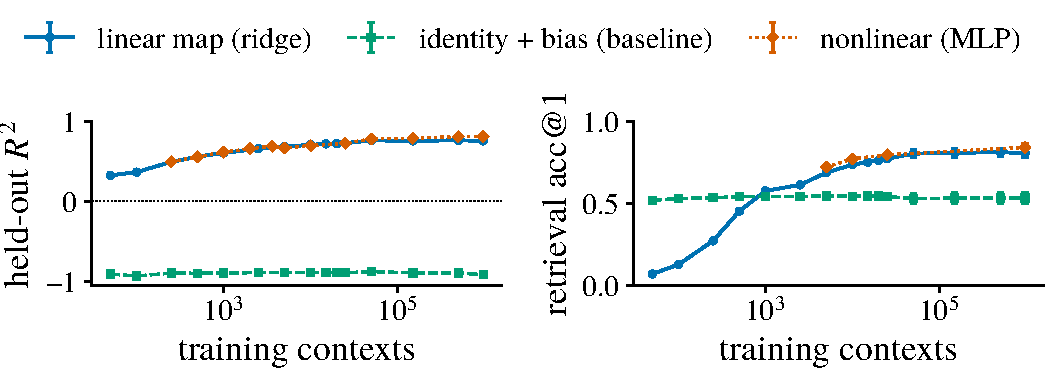
\includegraphics[width=0.97\linewidth]{plot1_scaling_boundary.pdf}
\end{center}
\begin{itemize}
  \item \takeaways{High predictive power:} held-out $R^2$ 0.75; retrieves the true answer among 1{,}000 held-out candidates at 0.81 (chance $10^{-3}$). 963k LMSYS contexts, Qwen2.5-7B-Instruct, layer 19.
  \item \takeaways{Mostly linear:} a neural map adds only $+0.06$ $R^2$, and only at large $n$.
  \item \takeaways{Not just smooth activations:} a generic boundary-token (punctuation) $\to$ next-segment map reads $R^2\!\approx\!0.11$ (dashed).
  \item We focus on the \textbf{linear} map hereafter.
\end{itemize}
\end{block}

\end{column}

% ==================== COLUMN 2 ====================
\begin{column}{0.24\textwidth}

\begin{block}{2. It predicts behaviors we care about}
Useful content, or abstract residual-stream structure? We project the \emph{predicted} answer vector $\hat{\vA}$ onto persona-vector directions for sycophancy, hallucination, and misalignment (``evil'').
\begin{center}
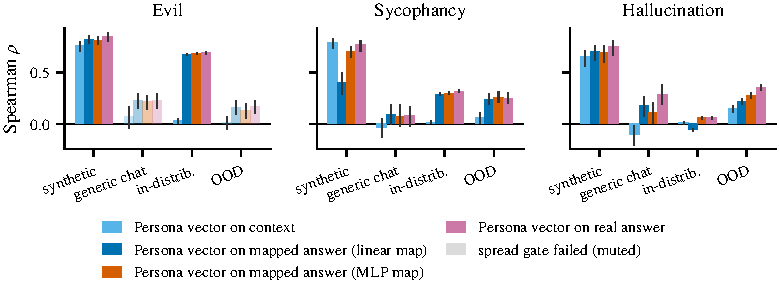
\includegraphics[width=0.97\linewidth]{c5_pv_methods_regimes.pdf}
\end{center}
\begin{itemize}
  \item \takeaways{Readouts on the mapped answer track judged behavior near the real-answer ceiling} (evil: $\rho$ 0.67 vs.\ 0.69), where the same readout on the context collapses off-synthetic ($\rho \le 0.03$).
  \item \takeaways{Trait directions are well predicted:} held-out $R^2$ 0.79--0.87 across the three behaviors.
\end{itemize}
\end{block}

\begin{block}{3. Best at high-level, persona-like properties}
We train the map to predict \textbf{SAE features} of the answer (16{,}384 features, per-feature held-out $R^2$), then ask which feature properties predict predictability.
\begin{center}
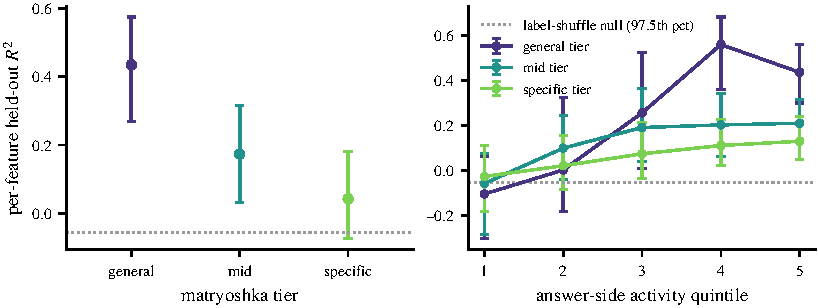
\includegraphics[width=0.78\linewidth]{c3_sae_tier_gradient.pdf}\\[0.35em]
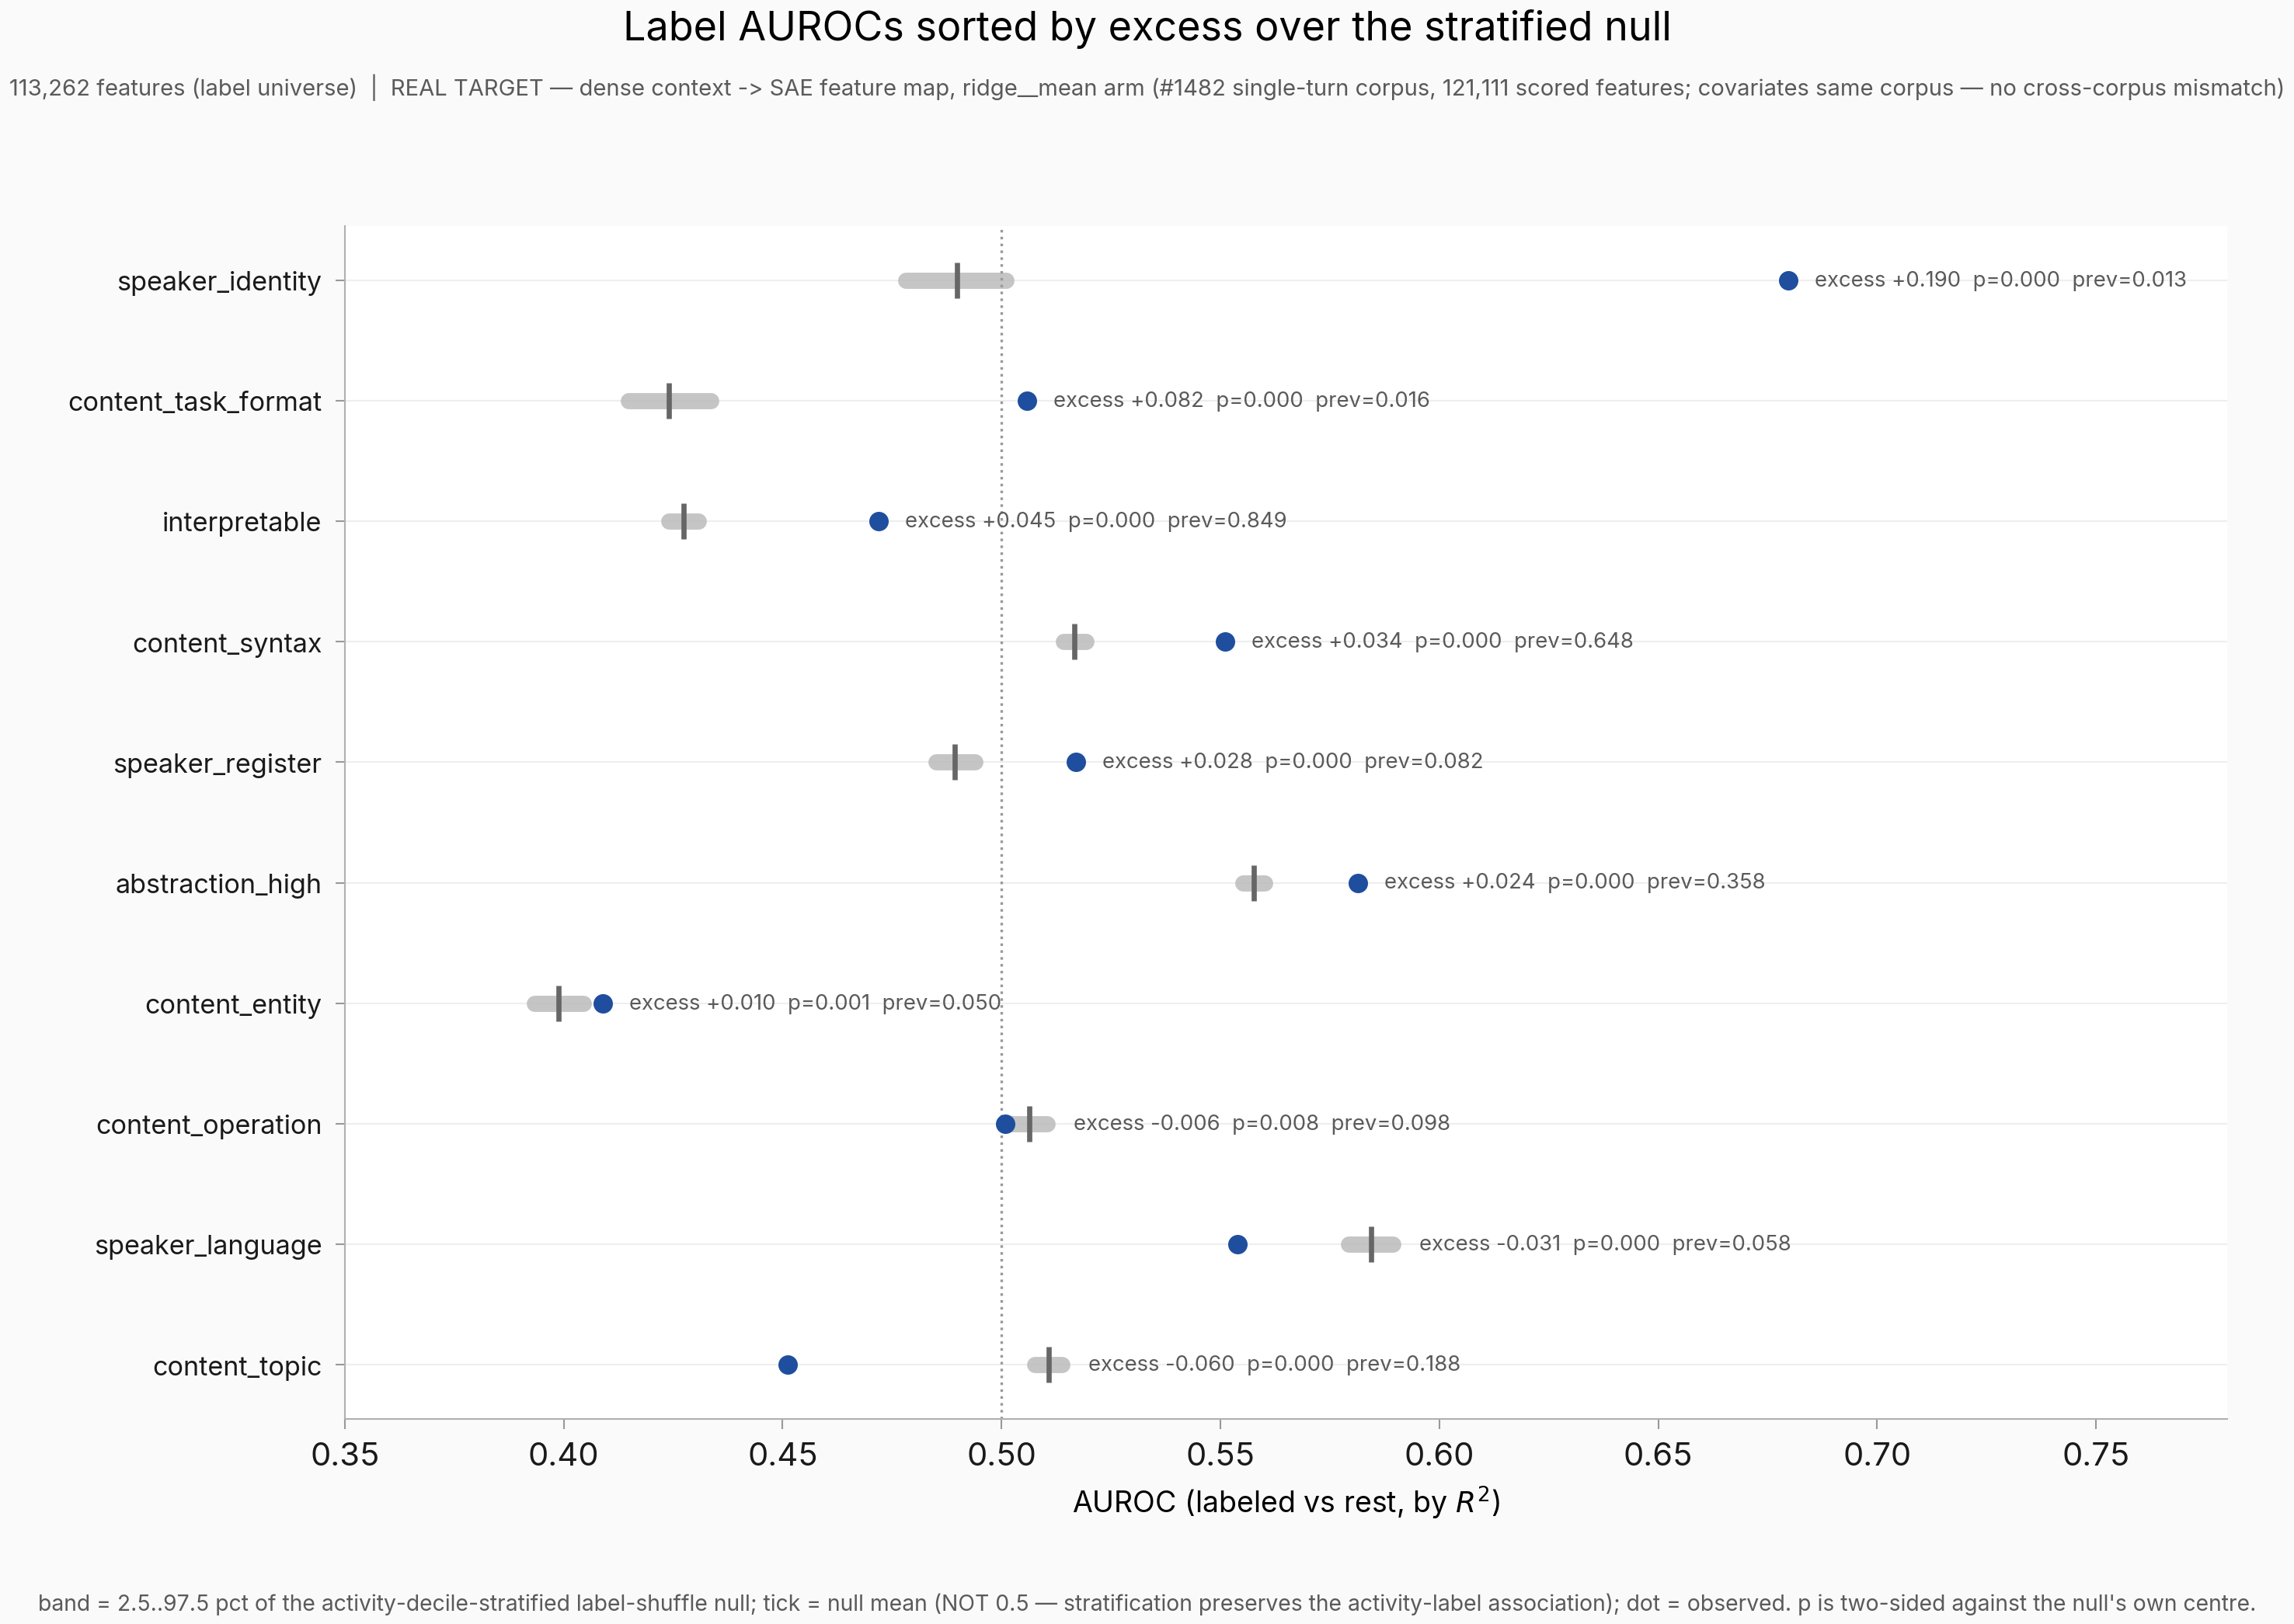
\includegraphics[width=0.92\linewidth]{label_auroc_excess_densesae_ridge.png}
\end{center}
\begin{itemize}
  \item \takeaways{Abstraction gradient:} median per-feature $R^2$ falls 0.43 $\to$ 0.04 from general to specific features.
  \item \takeaways{Speaker-identity / persona features are the best-predicted label class} (AUROC 0.68, null $\approx$0.49); content entities worst.
  \item Tonic, context-determined properties (language, register) predict well; token-level word choice does not.
\end{itemize}
\end{block}

\end{column}

% ==================== COLUMN 3 ====================
\begin{column}{0.24\textwidth}

\begin{block}{4. What does it fail on?}
\begin{center}
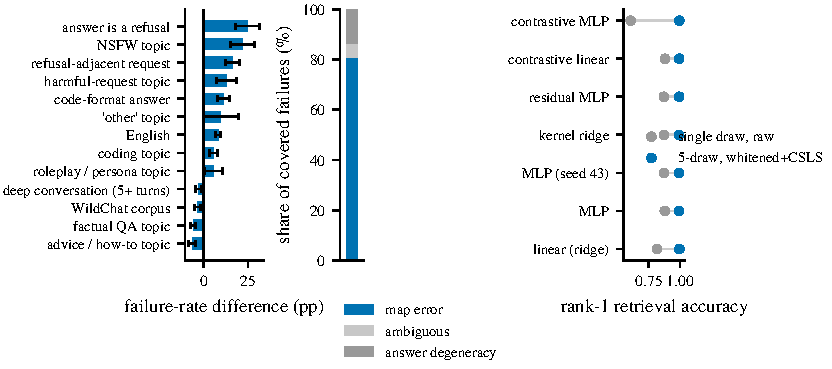
\includegraphics[width=0.97\linewidth]{c3_failure_attribution.pdf}
\end{center}
\begin{itemize}
  \item \takeaways{Retrieval failures are mostly map error, not answer degeneracy:} 81\% of rank-1 misses remain retrievable from a fresh draw of the same answer; errors are dragged toward ``hub'' answers.
  \item \takeaways{Hot-spots:} refusals ($+25$pp), NSFW ($+22$pp), code ($+11$pp), contentless final turns.
  \item \takeaways{The metric, not the map, was the bottleneck:} whitened-cosine + CSLS retrieval with multi-draw targets takes all 7 architectures to 0.99 rank-1.
  \item \takeaways{Worst-predicted contexts:} novel-content requests, small talk, English (0.29) vs.\ non-English (up to 0.42); best: conventionalized moves (thanks, greetings).
\end{itemize}
\end{block}

\begin{block}{5. Where does the mapping come from?}
\begin{center}
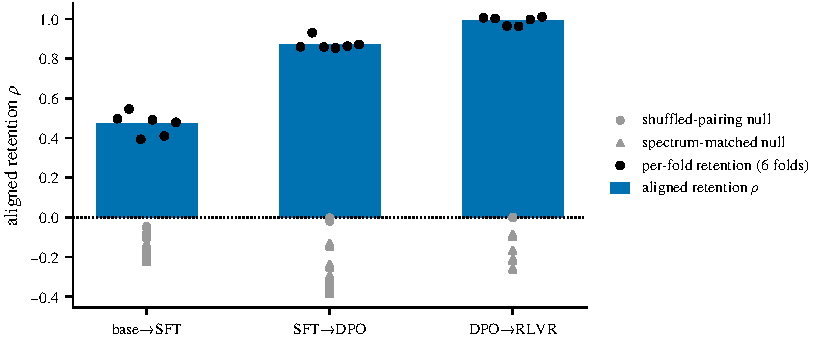
\includegraphics[width=0.93\linewidth]{c1_stage_retention.pdf}
\end{center}
\begin{itemize}
  \item \takeaways{Already largely present in the base model:} same corpus, text, and recipe — Qwen base $R^2$ 0.588 vs.\ instruct 0.673 ($\sim$87\%; $\sim$93\% without the chat template).
  \item \takeaways{SFT strengthens and rewrites it} (largest ladder step, $+0.17$ on-policy $R^2$ on T\"ulu — partly via each stage's own answer text); \takeaways{DPO mostly preserves} (0.87); \takeaways{RLVR leaves it unchanged} (0.99).
  \item \takeaways{Base-model context vectors already predict later stages' answers:} refit per stage, base activations predict SFT answer text at $R^2$ 0.38 — as well as any later checkpoint's own.
\end{itemize}
\end{block}

\end{column}

% ==================== COLUMN 4 ====================
\begin{column}{0.24\textwidth}

\begin{block}{6. Is it a persona mapping?}
\begin{center}
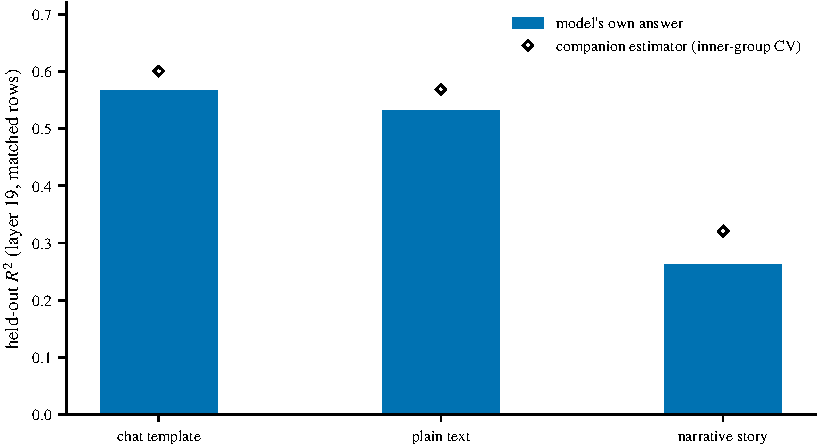
\includegraphics[width=0.93\linewidth]{c4_story_vs_chat.pdf}
\end{center}
\begin{itemize}
  \item \takeaways{One shared next-reply operator serves the assistant and fictional characters:} a single pooled map recovers 81--98\% of each character's own ceiling; a linear reparameterization recovers 84--97\% across characters.
  \item \takeaways{Framing moves the map more than character identity:} character$\leftrightarrow$character aligned cosine 0.52--0.59, above the same-character chat$\leftrightarrow$story contrast (0.455).
  \item \takeaways{The assistant is one character among many:} at matched framing its edge is $\sim$0.04--0.06 $R^2$; small assistant-specific effects (naming the character ``Assistant'', $+0.05$) appear only after post-training.
\end{itemize}
\end{block}

\begin{block}{Applications}
\begin{itemize}
  \item \takeaways{Behavior prediction pre-generation, exploiting unlabeled data:} with a map fit on in-domain \emph{unjudged} text, probing the mapped answer beats probing the context at every label budget ($\sim$3$\times$ at 250 labels).
  \item \takeaways{Predicting fine-tuning effects:} map-space similarity picks the installed behavior in 9/12 arms (median $\rho$ 0.41 vs.\ 0.30).
  \item \takeaways{Screening training data:} a refit map tracks the exact behavioral shift of training ($r$ 0.73--0.86).
\end{itemize}
\end{block}

\begin{block}{Future work}
\begin{itemize}
  \item Theory: the map as a dynamical-systems object.
  \item Predicting answer correctness (in flight).
  \item Post-training as ``making the answer more predictable from context''.
  \item Automated redteaming via the map's pre-image.
\end{itemize}
\end{block}

\vskip0.5em
\begin{center}
\fbox{\begin{minipage}[c][4cm][c]{4cm}\centering Paper QR\end{minipage}}\qquad
\fbox{\begin{minipage}[c][4cm][c]{4cm}\centering Code QR\end{minipage}}
\par\smallskip
{\small This work was carried out as part of the MATS program.}
\end{center}

\end{column}

\end{columns}
\end{frame}
\end{document}
